\section{SaUCy}
\label{sec:saucy}

Using ILC, we build a concrete, executable implementation of a simplified UC
framework, dubbed SaUCy. Then, we demonstrate the versatility of SaUCy in three
ways:
\begin{enumerate}[leftmargin=*]
\item We define a protocol composition operator and its associated composition theorem.
\item We walk through an instantiation of UC commitments.
\item We use ILC's type system to reason about ``reentrancy,'' a subtle definitional issue in UC that has only recently been studied.
\end{enumerate}


%\begin{figure}
%  \centering
%  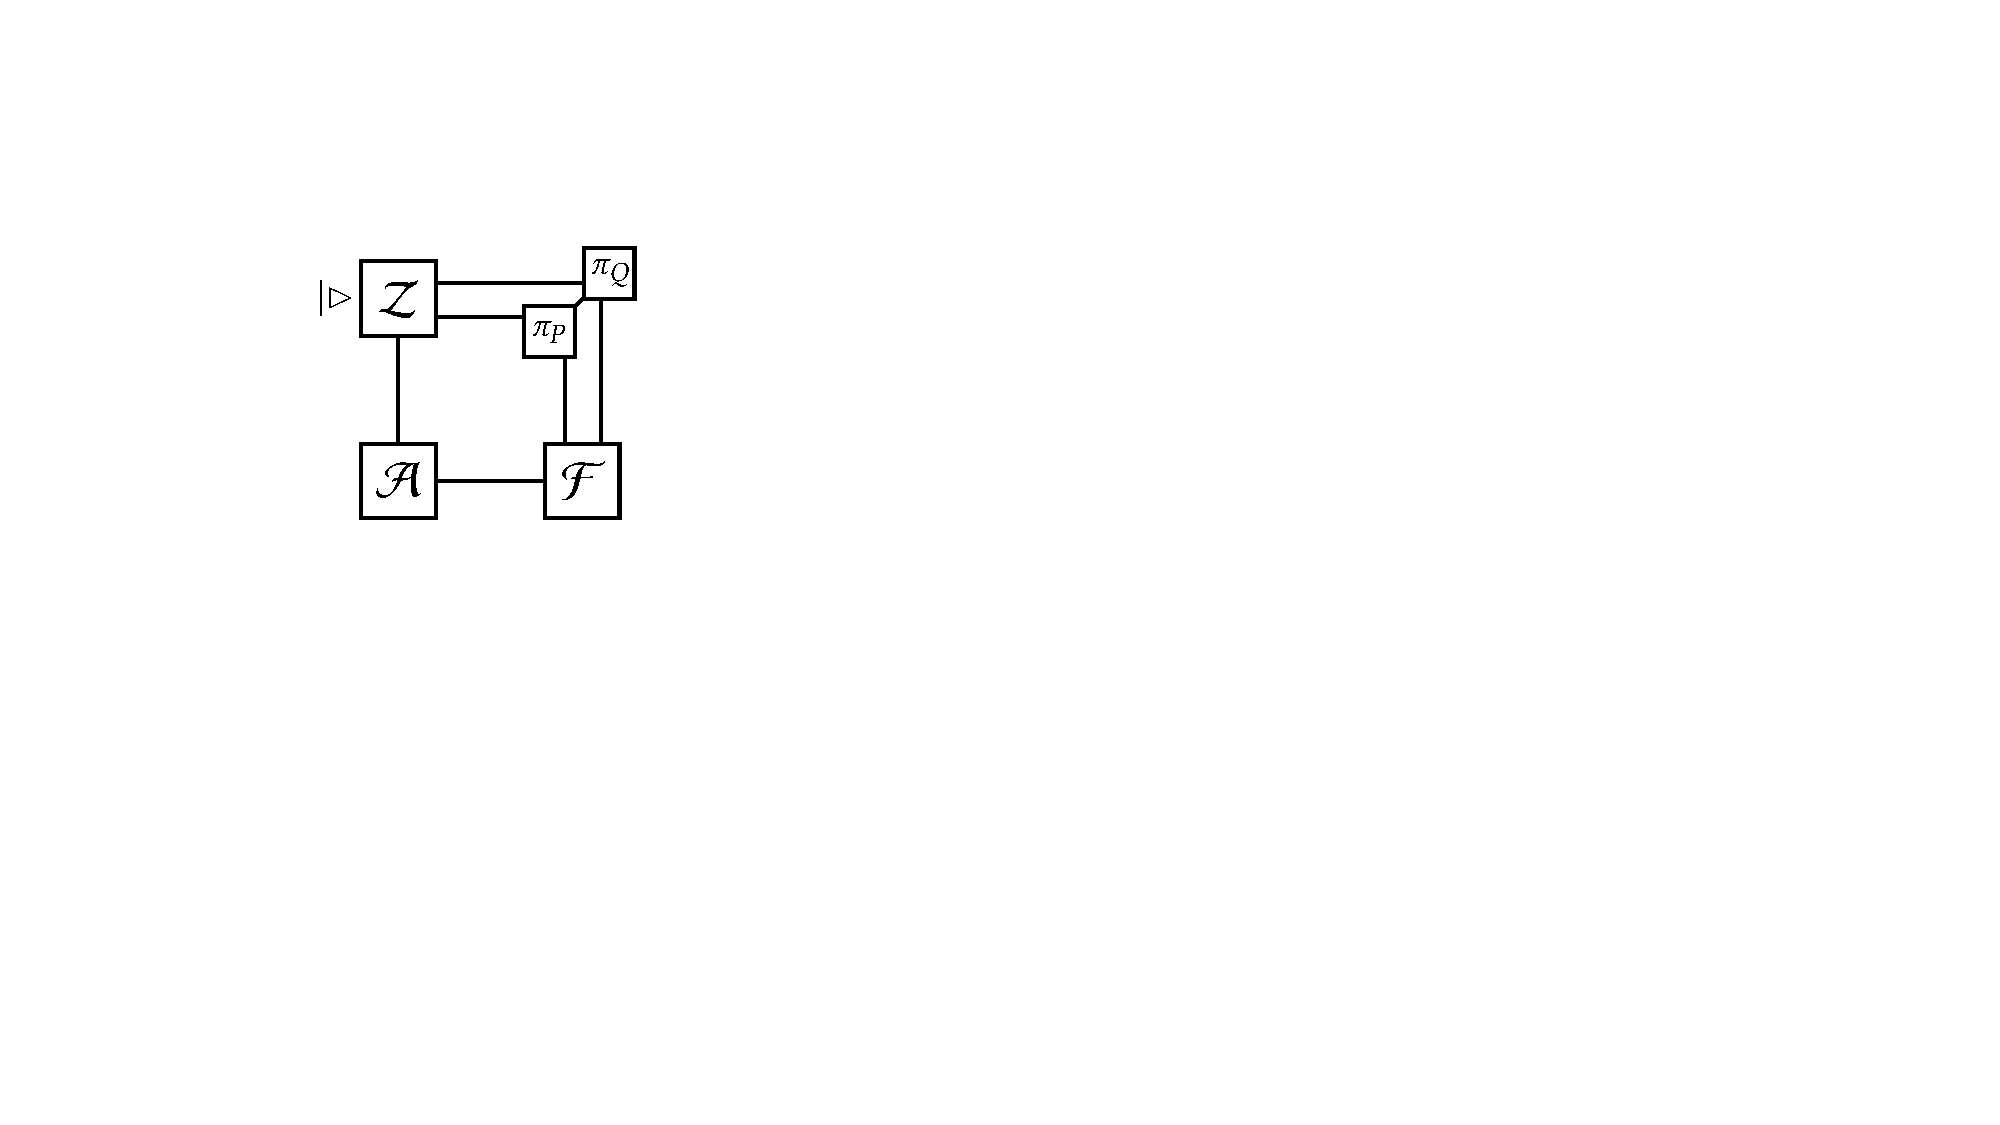
\includegraphics[width=0.4\linewidth]{graphics/execUC}
%  \caption{UC execution.}
%  \label{fig:execUC}
%\end{figure}


\subsection{Probabilistic Polynomial Time in ILC}
\label{subsec:ppt}
The goal of cryptography reduction is to relate every bad event in a protocol to
a \emph{probabilistic polynomial time computation} that solves a computationally
hard problem.  The ILC typing rules do not guarantee termination, let alone
polynomial time normalization, so we must tackle this in metatheory.  Also,
since ILC is effectively deterministic (confluent), we will need to express
random choices some other way.  To meet these needs, we define a judgment about
ILC terms that take a security parameter and a stream of random bits.

\begin{definition}[Polynomial time normalization]
  The judgment that $e$ is polynomial time normalizable, written $\mathsf{PPT}~e$, is defined as follows:
  \begin{mathpar}
    \Infer{ppt}
    {\emptyctxt; \emptyctxt |- e : \tyNat {->}\ [\tyBit] -> \tyBit\\
    \forall~k \in \tyNat.~\forall~r \in {[\tyBit]}^{\textnormal{poly}(k)}.~e~k~r~{->}^{\textnormal{poly}(k)}~v}
    {\keyword{PPT}~e }
  \end{mathpar}
  This says that if for all security parameters $k$ and all bitstrings $r$ (of
  length polynomial in $k$) the term $e~k~r$ normalizes to a value $v$ in
  $\textnormal{poly}(k)$ steps.
%  \footnote{Note that the normalization must be
%    polynomial time for all $\mathsf{r}$, though we could have defined it to
%    hold with high probability.}
\end{definition}

\todo{Other polynomial time notions.}

\begin{definition}[Value Distribution] 
  Because processes are confluent, we know that if $e~k~r~{->}^{*}~v$,
  then the value $v$ is unique.  We can therefore define the
  probability distribution ensemble
  $D(e) = \{ D_{e,k}\}_{k}$
  based on a uniform distribution $U_k$ over
  $k$-bit strings $r$, so the distribution $D_{e,k}$ is given as
\[
D_{e,k}(v) = \sum_{r \in R} U_{k}(r), \quad \textnormal{for~} R = \{ r ~|~ e~k~r~{->}^{*}~v \}.
\]
\end{definition}

\begin{definition}[Indistinguishability]
What remains is to define a notion of indistinguishability for value distributions. However, we need to clarify when polynomial time normalization is an assumption or a proof obligation.
  To simplify things later, we define a partial order $e_1 \le e_2$, which captures that $e_2$ must be $\mathsf{PPT}$ if $e_1$ is $\mathsf{PPT}$, and if so, that their value distributions are statistically similar.
  \begin{mathpar}
    \Infer{indist}
    {\keyword{PPT}~e_1 \implies (\keyword{PPT}~e_2 ~~\textnormal{and}~~
    {D(e_1) \sim D(e_2)})}
    {   \qquad e_1 \le e_2 }
  \end{mathpar}
\end{definition}

\subsection{SaUCy Execution Model}
\label{subsec:concrete-uc}
\begingroup
\setlength\intextsep{0pt}
\setlength{\columnsep}{10pt}
\begin{wrapfigure}{R}{0.15\textwidth}
\centering
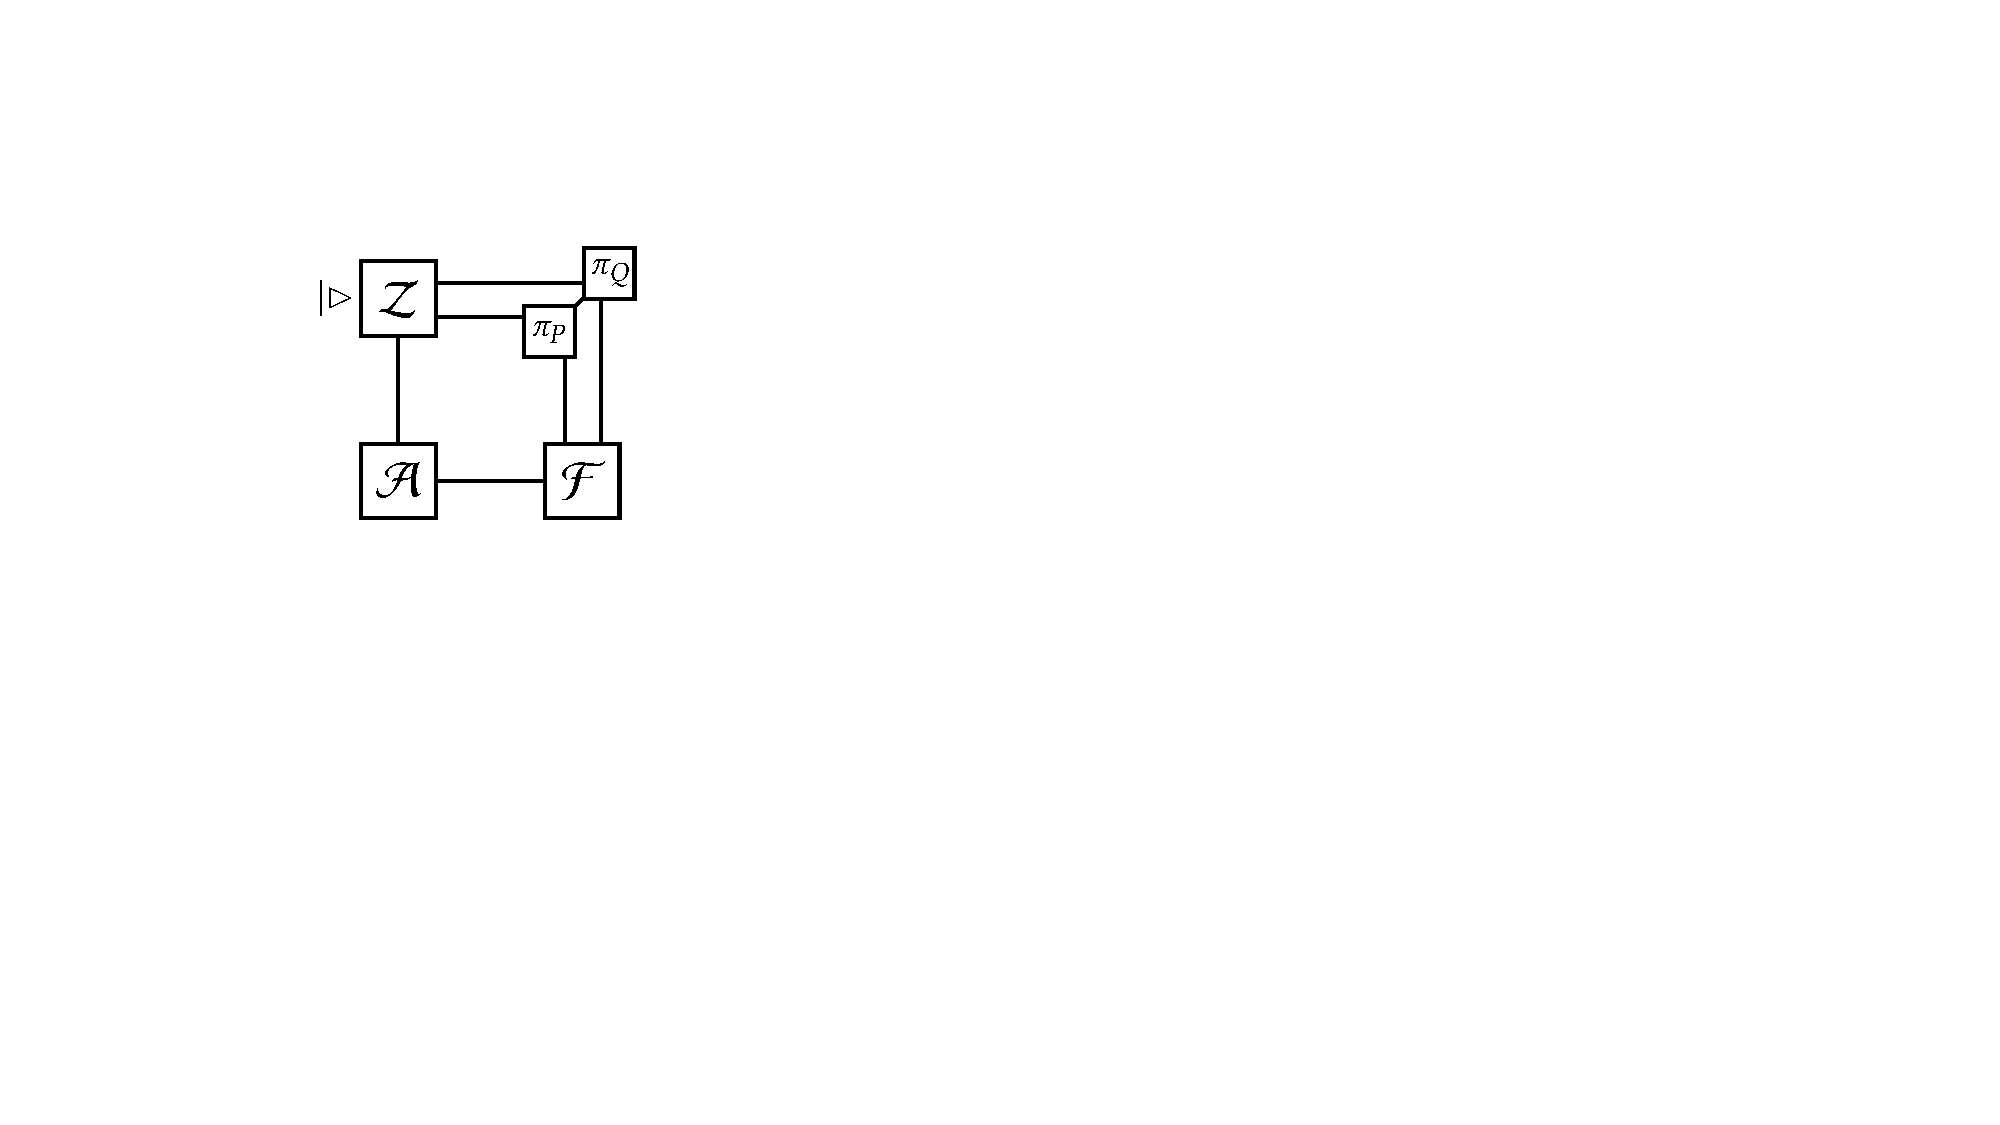
\includegraphics[width=0.15\textwidth]{graphics/execUC}
\caption{\textsf{execUC}.}
\label{fig:execUC-diagram}
\end{wrapfigure}
% \todo{``Too short to be useful'' needs more intuition, execUC abbreviation.}
% Two goals of this subsection:
% - give forward examples of main UC concepts to code in our example
% - identify and explain the simplifications in SaUCy
The implementation of SaUCy is centered around a definition of the UC execution
model in ILC.  The full code listing of \textsf{execUC} is given in the
Appendix.  For the most part, \textsf{execUC} just involves connecting channels
as illustrated in Figure~\ref{fig:execUC-diagram}.  The execution is centered on
the environment $\mc{Z}$, in the sense that $\mc{Z}$ first gets the write token,
and the experiment concludes when $\mc{Z}$ returns a value.  Apart from this, we
explain some of our main modeling choices and the consequences they have for the
ILC implementation.

To start with, we make several simplifications to standard UC, for example
focusing on the special case of two-party protocols (\`{a} la Simplified
UC~\cite{canetti2015simpler}).  We also only aim to show the case of
\emph{static} corruptions, in which the corrupt parties are determined at the
onset.  This is achieved by parameterizing the entire experiment by a value
\textsf{crupt :: Crupt}.  For a more general model with adaptive corruptions,
\textsf{execUC} would need to accept requests from the environment to add to the
\textsf{crupt} list as the execution proceeds.

Our corruption model is Byzantine, meaning the adversary gets to exert complete
control over the corrupted parties.
% There is an alternative way to implement this. Since the ideal functionality is also aware of \textsf{crupt}, it can present an ``adversary interface,'' and accept commands on behalf of honest parties anyway.
For each party, depending on the value of \textsf{crupt}, either we run a copy
of the honest protocol, or connect the channels to the adversary. This is
implemented in the function \textsf{corruptOrNot}.
%are two cases: corrupt (the adversary controls them), or honest (they follow the
%protocol). This logic is captured by an ILC \textsf{wrapper} function (shown in
%the Appendix).

%\lstinputlisting[style=myilc]{listings/simp-suc.ilc}
% data Crupt = CruptP | CruptQ | CruptNone
% which
% will suffice for our example of instantiating universally composable
% commitments.

We also model a strong form of communication channels between the parties: $P$
and $Q$ are connected by a pair of raw ILC channels. Communication over these
channels happens immediately, without activating the adversary or leaking even
the existence of the message.  In a more realistic model, the parties would only
be able to communicate over a network channel modeled as a functionality,
$\F{\textsc{smt}}$ or $\F{\textsc{syn}}$~\cite{canetti2001universally}.
Consequently our $\F{\textsc{com}}$ functionality would need to be weakened by
leaking some (model-specific) information about the message to the adversary.

%\noindent The function \textsf{execUC} is parameterized by an environment \textsf{z},
%protocol parties \textsf{p} and \textsf{q}, an adversary \textsf{a}, an ideal
%functionality \textsf{f}, a security parameter \textsf{k}, a random bitstring
%\textsf{r}, and a static corruption model \textsf{crupt :: Crupt}.
%\textsf{Crupt} datatype is defined below, with its variants denoting the cases
%when party \textsf{p} is corrupt, party \textsf{q} is corrupt, or no party is
%corrupt, respectively.
%\lstinputlisting[style=myilc]{listings/crupt.ilc}
%\endgroup

% Note that for space and readability, we elide channel allocation/distribution
% and wrapper definitions (with ellipses). We also abbreviate the type signature
% (e.g., $A_{\mathsf{z}}$ is the type of \textsf{z}). More details can be found in
% the Appendix.
%Note that for space and readability, we elide channel allocation/distribution
%with ellipses. We also abbreviate the type signature (e.g., $A_{\mathsf{z}}$ is
%the type of \textsf{z}). More details can be found in the Appendix.

\begin{comment}
\begin{itemize}[leftmargin=*]
  \item \emph{Environment.} The environment's program defines interactions with
    the protocol parties and the adversary, which have different programs in the
    real world and the ideal world (see below). Its job is to distinguish which
    of the worlds it is interacting with.
  \item \emph{Protocol.} In the real world, the program of the protocol parties
    correspond to actual programs for running the protocol. In the ideal world,
    the protocol parties are simply dummy parties, which relay messages between
    the environment and the functionality.
  \item \emph{Adversary.} In the real world, the adversary is simply the dummy
    adversary, which relays messages between the environment and either the
    functionality or a corrupted party. In the ideal world, the adversary is a
    simulator, which must mimic the attack of any real world adversary, but in
    the ideal world.
  \item \emph{Functionality.} In the real world, the functionality is any
    functionality that the real world protocol makes calls to (if any). In the
    ideal world, the functionality is the specification for the protocol under
    analysis.
  \item \emph{Security parameter.} Each process is handed a security parameter
    (a natural number), and must run in a number of steps polynomial in this
    security parameter. We have more to say on this later.
  \item \emph{Corruptions.} The possible corruption models are either party
    \textsf{p} is corrupt, party \textsf{q} is corrupt, or no parties are
    corrupt, which are defined in the following datatype:
    \lstinputlisting[style=myilc]{listings/crupt.ilc}
\end{itemize}
\end{comment}

%For a real world execution, the protocol parties contain code for running the
%actual protocol under analysis, the adversary is the dummy adversary, and the
%ideal functionality is any functionality that the protocol makes calls to (if
%any). For an ideal world execution, the protocol parties are simply dummy
%parties, the adversary is a simulator, and the ideal functionality is a
%specification for the protocol under analysis. The environment has the ability
%to interact with each of the executions as they evolve. For the simulation to be
%good, the environment should not be able to distinguish which of the executions
%it is interacting with.


\subsection{Defining UC Security in ILC}
\label{subsec:uc}
The central security definition in UC is protocol emulation.  The guiding
principle is that $\pi$ emulates $\phi$ if the environment cannot distinguish between
the two protocols.  Our first attempt is the following, where $\mc{S}$ is the
simulator that translates every attack in the real world into an attack
expressed in the ideal world:
\begin{mathpar}
  \Infer{\st{emulate}}
        {\forall~\mc{Z}.~ 
         \mathsf{execUC}\ \mc{Z}\ \pi\ \mc{F}_1\ {\mathbbm{1}}_\mc{A} \le
         \mathsf{execUC}\ \mc{Z}\ \phi\ \mc{F}_2\ \mc{S}}
    {\mc{S} \entails (\pi, \mc{F}_1) \approx (\phi, \mc{F}_2)}
\end{mathpar}
To remark on a few notation choices: we make the functionality explicit, so emulation
is a relationship between protocol-functionality pairs.  Here,
$\mathbbm{1}_\mc{A}$ is the dummy adversary, which just relays messages between
the environment and the parties/functionality. We elide the standard dummy lemma that shows
this is without loss of generality; the intuition is that whatever an adversary
can do, the environment can achieve using $\mathbbm{1}_\mc{A}$.

%\[
%(\pi, \mc{F}_1) \overset{\mc{S}} \le (\phi, \mc{F}_2)
%\]
%\[
%S ~\keyword{proves}~ (\pi, \mc{F}_1) ~\keyword{emulates}~ (\phi, \mc{F}_2).
%  \]
%  Since the simulator tranlates attacks $\mc{A}$ to the real world, we treat $\mc{S}$ as a function, so $\mc{S A}$ is the ideal world adversary simulating $\mc{A}$.

%% Since emulation means that any attack on $\pi$ is also on $\phi$.
%% We have to translate \emph{attacker behaviors} of an arbitrary real world adversary $\mc{A}$ to a simulated adversary $\mc{(S~A)}$ in the ideal world.

Unfortunately this simple definition turns out to be vacuous: a degenerate
protocol $\pi$ can emulate anything simply failing to be $\keyword{PPT}$, e.g. by
diverging. To put it another way, the problem is the definition imposes a proof
obligation on the simulator $\mc{S}$ but not on $\pi$.  What we want to say is
that the \emph{real world} protocol $(\pi, \mc{F}_1)$ must be well behaved
whenever the \emph{ideal world} $(\phi, \mc{F}_2)$ is.  However, even a reasonable
protocol can result in non-PPT executions if paired with a divergent
environment.  In fact, giving a precise but composable notion of polynomial-time
for interactive processes has been an ongoing challenge in UC. In GNUC, the
approach is to define a well behaved environment, independently of its execution
context---roughly that the total size of its outgoing messages is bounded by a
polynomial, and that its running time is bounded if its total received input
size is bounded~\cite{hofheinz2015gnuc}. This notion is composable as desired,
although its use requires additional distinctions between ``invited'' and
``uninvited'' messages. RSIM makes analogous
choices~\cite{backes2007reactive}. While we think these could be equally applied
to ILC, for example, through refinement types \`{a} la the RCF
calculus~\cite{bugliesi2015affine}, our goal here is to provide a simpler
notion.

We define protocol emulation by requiring a simulation in both directions, so
every behavior in the ideal world must correspond to a behavior in the real
world and vice versa.
\begin{definition}[Protocol Emulation]
  The judgment that one protocol-functionality pair $(\pi, \mc{F}_1)$ securely
  emulates another $(\phi, \mc{F}_2)$ (as proven by the simulators
  $\mc{S}_\mc{R},\mc{S}_\mc{I}$) is defined as
\begin{mathpar}
  \Infer{{emulate}}
        {\forall~\mc{Z}.~ 
         \mathsf{execUC}\ \mc{Z}\ \phi\ \mc{F}_2\ \mathbbm{1}_\mc{A} \le
         \mathsf{execUC}\ \mc{Z}\ \pi\ \mc{F}_1\ \mc{S_\mc{R}} \\\\
         \ \ \ \ \ \ \ \ ~\mathsf{execUC}\ \mc{Z}\ \pi\ \mc{F}_1\ \mathbbm{1}_\mc{A} \le
         \mathsf{execUC}\ \mc{Z}\ \phi\ \mc{F}_2\ \mc{S}_\mc{I}}
    {\mc{S_\mc{R},S_\mc{I}} \entails (\pi, \mc{F}_1) \approx (\phi, \mc{F}_2)}
\end{mathpar}
\end{definition}
\noindent We remark this definition goes against the UC convention of requiring
simulation in one direction only. One direction is preferable intuitively
because it should be fine if the protocol is even more secure than its
specification.
This does not pose any problem for our commitment example; however, a protocol that leaks even less information than the ideal functionality requires could be difficult to prove under this definition.
In any case, the benefit is this
simplifies the polynomial time notion: vacuous protocols are clearly ruled out
by the top condition, and both simulations are only required to be \keyword{PPT}
if $\mc{Z}$ is.

%%   \begin{mathpar}
%%   \Infer{\st{emulate}}
%%         {\forall~\mc{A}~\mc{Z}.~ \keyword{PPT}~(\mathsf{execUC}~\mc{Z}~\phi~1_\mc{A}~\mc{F}_2) => \\\\
%%   \keyword{PPT}~(\mathsf{execUC}~\mc{Z}~\pi~\mc{S_\mc{R}}~\mc{F}_1)
%% \\\\
%%          \mathsf{execUC}\ \mc{Z}\ \pi\ \mc{F}_1\ \mc{A} \le
%%          \mathsf{execUC}\ \mc{Z}\ \phi\ \mc{F}_2\ (\mc{S}~\mc{A})}
%%         {(\pi, \mc{F}_1) \overset{\mc{S}}\le (\phi, \mc{F}_2)}
%%   \end{mathpar}
  

%
%
%We therefore need to express a judgment $\keyword{Good}$ to describe environments that are well behaved in the ideal world:
%\begin{mathpar}
%  \Infer{good}
%        {\keyword{PPT}~(\mathsf{execUC}~\mc{Z}~\phi~1_\mc{A}~\mc{F}_2)}
%        {\keyword{Good}~\phi~\mc{F}_2~\mc{Z}}
%\end{mathpar}
%% To resolve this concern, we say that every \emph{benign behavior} in the ideal world must translate to. We require an additional simulator in the real world $\mc{S_\mc{R}}$      says that every benign behavior in the ideal world must correspond to a benign environment in the real world. To characteris
%% \noindent Notice that this constraint has the dummy adversary $1_\mc{A}$.
%% %, even though it is written for the ideal world, unlike in the dummy lemma.
%% This is without loss of generality in the sense that $\keyword{Good}~\phi~\mc{F}_2~Z$ implies that for any $\mc{A}$, we could have a $\mc{Z'}$ such that
%% \[
%% \mathsf{execUC}~\mc{Z} ~\phi  ~\mc{A}~\mc{F}_2 \le
%% \mathsf{execUC}~\mc{Z'}~\phi~1_\mc{A}~\mc{F}_2
%% \]


\subsection{A Composition Theorem in SaUCy}
\label{subsec:composition}

%\begin{figure}
%  \centering
%  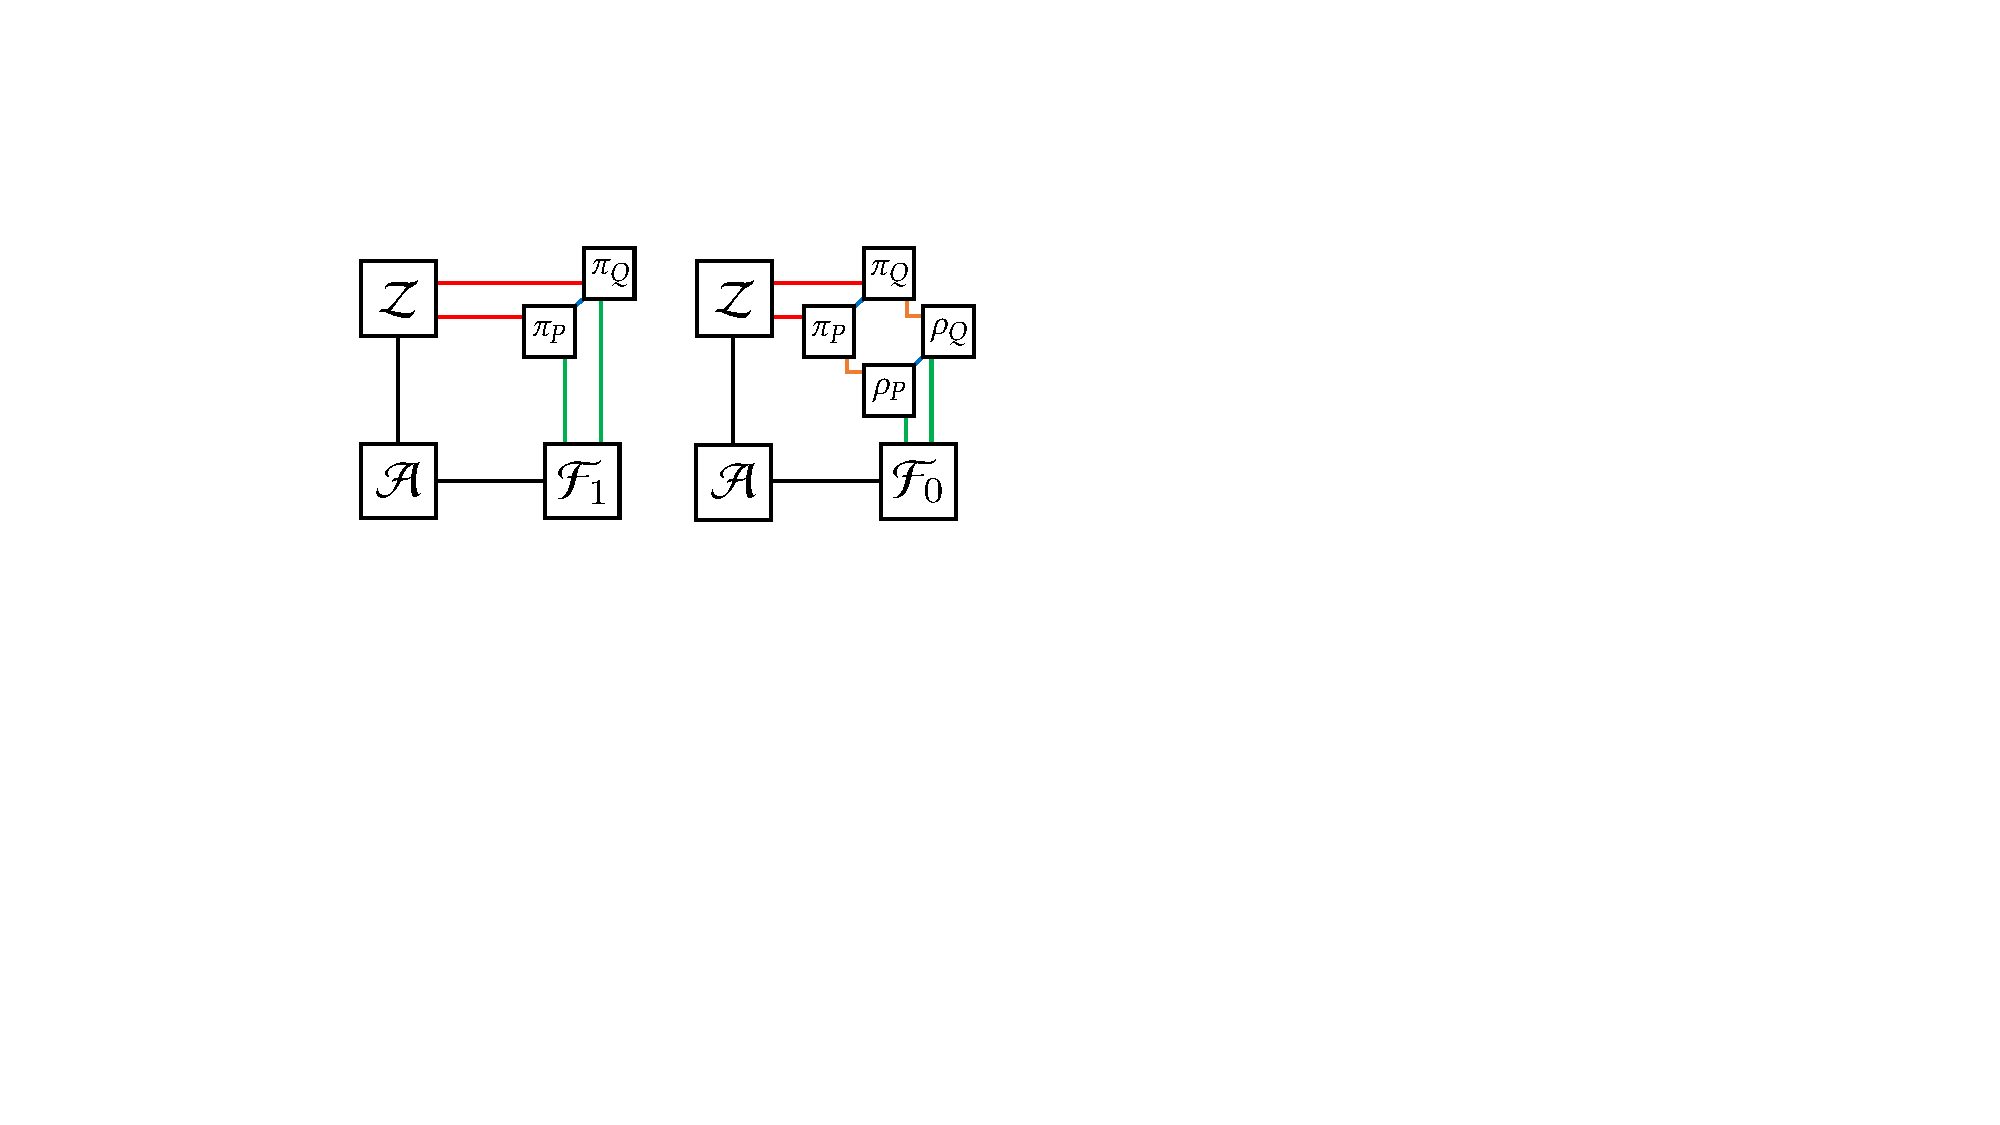
\includegraphics[width=0.75\linewidth]{graphics/protocol-composition}
%  \caption{Protocol composition diagram.}
%  \label{fig:protocol-composition}
%\end{figure}

As a first demonstration of SaUCy, we work through the development of a composition
operator, and give a theorem explaining its use.
\begin{definition}[UC realizes]
To set out, we introduce the notation of ``realizes,'' which views a protocol as a way of instantiating a specification functionality $\mc{F}_{2}$ from a setup assumption functionality $\mc{F}_1$,
%  if $\keyword(\mc{Z}, \pi, \mc{F}_0, \mc{A}_{\mathbbm{1}})$, then
%  $|- \keyword{polyUC}(\mc{Z}, \pi_{\mathbbm{1}}, \mc{F}_1, \mc{S})$, and the
  %  following statistical indistinguishability relation holds
\begin{mathpar}
  \Infer{realizes}
  {(\pi,~\mc{F}_1) \approx (\mathsf{id}_\pi, \mc{F}_2)}
  {\mc{F}_1 \yrightarrow{$\pi$} \mc{F}_2}
  \end{mathpar}
\end{definition}
\noindent where $\mathsf{id}_\pi$ is the \emph{dummy protocol}, which simply relays messages between the environment and the functionality.
This notation is convenient because it suggests a categorical approach to composition.

\begin{theorem}[Composition Theorem]
  \begin{mathpar}
  \Infer{}
  {\mc{F}_1 \yrightarrow{$\pi$} \mc{F}_2 \\ 
  \mc{F}_2 \yrightarrow{$\rho$} \mc{F}_3}
  {\mc{F}_1 \yrightarrow{$\rho \circ \pi$} \mc{F}_3}
  \end{mathpar}
\end{theorem}

\noindent The idea is that the $\rho \circ \pi$ can be defined in a natural way, where the ideal
functionality channel of $\rho$ is connected to the environment channel of $\pi$, as
illustrated and defined in Figure~\ref{fig:composition-operator}.
\begin{figure}
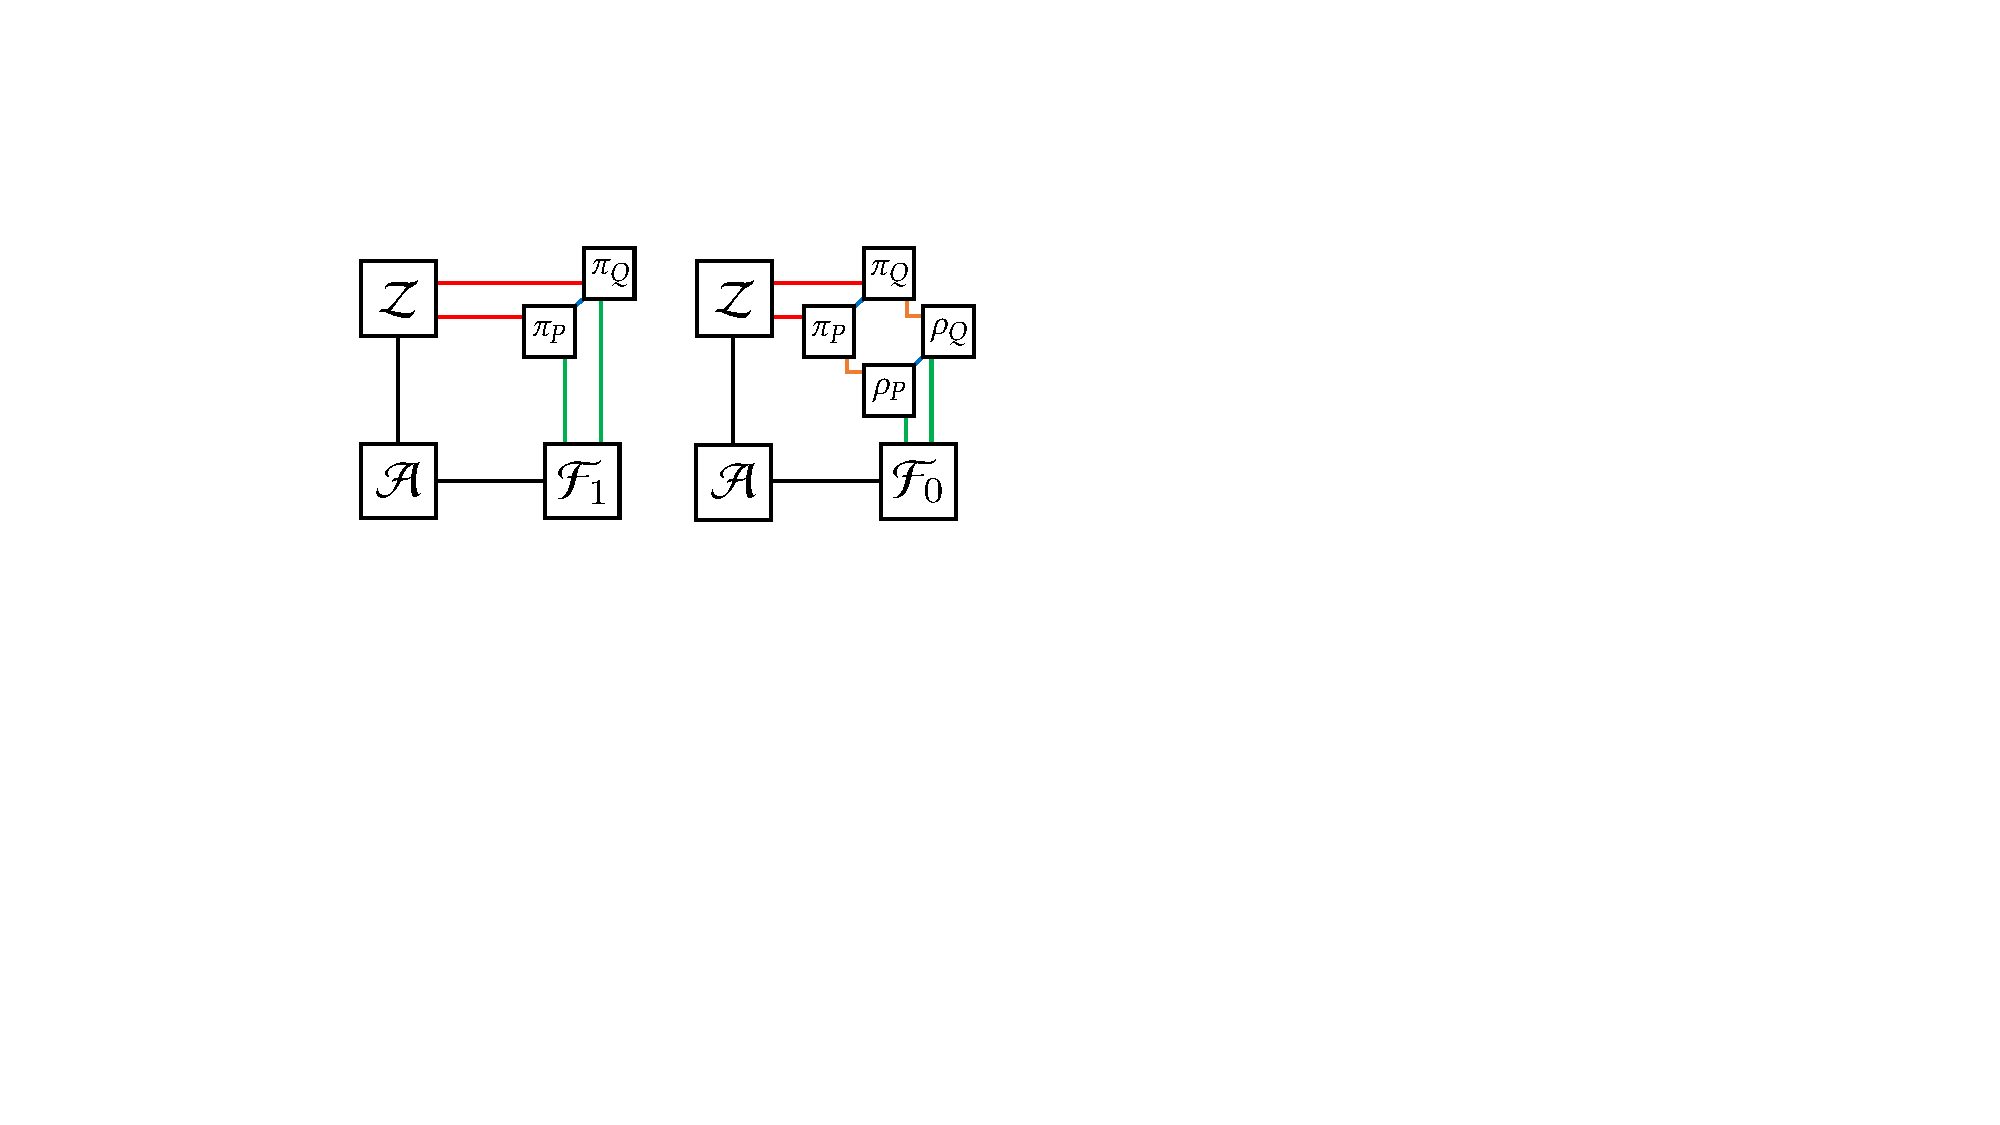
\includegraphics[width=0.6\linewidth]{graphics/protocol-composition}
\lstinputlisting[style=myilc]{listings/compose.ilc}
\caption{Protocol composition operator.}
\label{fig:composition-operator}
% The following is the nu block
  % (${\color{orange}\sf r{\rho_P}2{\pi_P}}$, ${\color{orange}\sf w{\rho_P}2{\pi_P}}$), (${\color{orange}\sf r{\pi_P}2{\rho_P}}$, ${\color{orange}\sf w{\pi_P}2{\rho_P}}$)
  % , (${\color{orange}\sf r{\rho_Q}2{\pi_Q}}$, ${\color{orange}\sf w{\rho_Q}2{\pi_Q}}$), (${\color{orange}\sf r{\pi_Q}2{\rho_Q}}$, ${\color{orange}\sf w{\pi_Q}2{\rho_Q}}$)
  % , (${\color{blue}\sf r{\rho_P}2{\rho_Q}}$, ${\color{blue}\sf w{\rho_Q}2{\rho_Q}}$), (${\color{blue}\sf r{\rho_Q}2{\rho_P}}$, ${\color{blue}\sf w{\rho_Q}2{\rho_Q}}$)		  

\end{figure}

\noindent \proof To prove the theorem we construct the simulators $S_{\mc{R},\rho} \circ S_{\mc{R},\pi}$ (respectively $S_{\mc{I},\rho} \circ S_{\mc{I,\pi}}$) in the natural way as well (given in the Appendix).
Our proof obligation is to introduce an arbitrary environment $\mc{Z}$ and conclude
\[  \keyword{execUC}~\mc{Z} ~(\rho \circ \pi)~\mc{F}_1 ~\mathbbm{1}_\mc{A}
\le \keyword{execUC}~\mc{Z} ~\mathbbm{1}_\mc{\pi} ~\mc{F}_3 ~(\mc{S}_{\mc{I},\rho} \circ \mc{S}_{\mc{I},\pi})
.\]
\noindent
%
The main idea is to notice that that we can bring $\rho$ from the composed protocol into the environment as $(\mc{Z}\circ \rho)$, reflecting the fact that the environment is meant to represent arbitrary outer protocols. The following derivation completes the proof:
\begin{align*}
    &~ \keyword{execUC}~\mc{Z}~(\rho \circ \pi)~\mc{F}_1~ \mathbbm{1}_\mc{A} & \\
  = &~ \keyword{execUC}~(\mc{Z}\circ \rho)~\pi~\mc{F}_1~ \mathbbm{1}_\mc{A} &
  \textnormal{(By inspection)} \\
\le&~ \keyword{execUC}~(\mc{Z}\circ \rho)~\mathsf{id}_\pi ~\mc{F}_2~ \mc{S}_{\mc{I},\pi} & (\textnormal{From}~ \mc{F}_1 \yrightarrow{$\pi$} \mc{F}_2) \\
 = &~ \keyword{execUC}~(\mc{S}_{\mc{I},\pi}\circ \mc{Z})~\rho ~\mc{F}_2~ \mathbbm{1}_\mc{A} &  \textnormal{(By inspection)} \\
\le&~ \keyword{execUC}~(\mc{S}_{\mc{I},\pi}\circ\mc{Z})~\mathsf{id}_\pi~\mc{F}_3~\mc{S}_{\mc{I},\rho} &
(\textnormal{From}~ \mc{F}_2 \yrightarrow{$\rho$} \mc{F}_3) \\
= &~ \keyword{execUC}~\mc{Z}~ \mathsf{id}_\pi~ \mc{F}_3~ (\mc{S}_{\mc{I},\pi} \circ \mc{S}_{\mc{I},\rho}) &
\textnormal{(By inspection)}
\end{align*}
The remaining case for $\mc{S}_{\mc{R},\rho} \circ \mc{S}_{\mc{R},\pi}$ is symmetric.\qed
\begin{comment}
The following equivalence is clear:
\begin{equation}
   \keyword{execUC}~\mc{Z}~(\rho \circ \pi)~\mc{F}_1~ \mathbbm{1}_\mc{A} =
   \keyword{execUC}~(\mc{Z}\circ \rho)~\pi~\mc{F}_1~ \mathbbm{1}_\mc{A}
\end{equation}

%% (1) Notice that by code path tracing equality:
%% execUC Z φπ F1 1 =
%% execUC (Z φ) π F1 1

Next, from $\mc{F}_1 \yrightarrow{$\pi$} \mc{F}_2$ we know %
\begin{equation}
  \keyword{execUC}~(\mc{Z}\circ \rho)~\pi~\mc{F}_1 ~ \mathbbm{1}_\mc{A} \le
  \keyword{execUC}~(\mc{Z}\circ \rho)~\mathsf{id}_\pi ~\mc{F}_2~ \mc{S}_{\mc{I},\pi}
\end{equation}
%% (2) Load (A) to have
%% execUC (Z φ) π F1 1 ≤ execUC (Z φ) 1 F2 SI1

Again by equality, we can see:
\begin{equation}
  \keyword{execUC}~(\mc{Z}\circ \rho)~\mathsf{id}_\pi~\mc{F}_2 ~ \mc{S}_{\mc{I},\pi} =
  \keyword{execUC}~(\mc{S}_{\mc{I},\pi}\circ \mc{Z})~\rho ~\mc{F}_2~ \mathbbm{1}_\mc{A}
\end{equation}
%% (3) Notice that by code path tracing equality:
%% execUC (Z φ) 1 F2 SI1 =
%% execUC (SI1 Z) φ F2 1

Next, from $\mc{F}_2 \yrightarrow{$\rho$} \mc{F}_3$ we know %
\begin{equation}
   \keyword{execUC}~(\mc{S}_{\mc{I},\pi}\circ\mc{Z})~\rho~ \mc{F}_2~\mathbbm{1}_\mc{A}
\le\keyword{execUC}~(\mc{S}_{\mc{I},\pi}\circ\mc{Z})~\mathsf{id}_\pi~\mc{F}_3~\mc{S}_{\mc{I},\rho}
\end{equation}
%% (4) Load (B) to have
%% execUC (SI1 Z) φ F2 1 ≤ execUC (SI1 Z) 1 F3 SI2

Finally, again by equality:
\begin{equation}
  \keyword{execUC}~(\mc{S}_{\mc{I},\pi}~\mc{Z})~\mathsf{id}_\pi~\mc{F}_3~\mc{S}_{\mc{I},\rho} =\keyword{execUC}~\mc{Z}~ \mathsf{id}_\pi~ \mc{F}_3~ (\mc{S}_{\mc{I},\pi} \circ \mc{S}_{\mc{I},\rho})
\end{equation}
\end{comment}
%% (5) By equality:
%% execUC (SI1 Z) 1 F3 SI2 =
%% execUC Z 1 F3 (SI1 o SI2)

\paragraph{Other notions of composition.}
Our composition operator above is just a starting point.
The ``universal composition''~\cite{canetti2001universally} operator essentially multiplexes sessions identified by unique tags (\emph{session ids}), while a joint state composition theorem collapses multiple subroutines into one~\cite{canetti2003universal}.
Despite its name, development in UC often involves defining additional composition operators. 
For example, interesting composition often happens ``in the functionality''
through higher order ``wrapper''
functionalities~\cite{kosba2016hawk,katz2007universally} which we would express
through abstraction. Some security properties require a generalized notion of
ideal functionality that the environment can interact with directly. All the
above motivate the development of the ILC core calculus as a flexible
foundation; developing them in ILC is important future work. \todo{Comparison}


\subsection{Instantiating UC Commitments}
\label{subsec:example}
We next walk through an instantiation of UC commitments (\`{a} la Canetti and
Fischlin~\cite{canetti2001commitments}).
Instantiation proofs in SaUCy follow a
standard rhythm. We start with a security definition as an ideal functionality
(such as $\Func_{\textsc{com}}$), give the protocol, construct a simulator, and
finally complete the relational analysis on paper.

Commitments are one of the simplest UC primitives, though as a case study this serves two main purposes.
First, the proof demonstrates several representative UC techniques~\cite{lindell2017simulate}, in particular the simulator makes use of a ``trusted setup'' and extracts inputs from a corrupt sender.
%The simulator's proof obligation is to use this trapdoor to simulate and extract.
Second, the protocol makes use of computational primitives and thus requires a reduction step in the proof, which can go through because of ILC's confluent design.

% Commitments are a simple functionality.
% We choose this because it illustrates a common pattern.
% The simulator makes use of trapdoor information contained within a CRS "trusted setup". The simulator uses this to extract (which enforces the soundness property) or to simulate a fake proof (which corresponds to the zero knowledge property).
% In this way commitments exercise the main path of a constructive proof.

% The second reason is that the commitment protocol relies on a computational primitive, pseudorandom function, and hence the relational analysis requires a computational reduction, would be difficult to express directly.

% TODO: Need a transition into the next paragraph
\paragraph{Extending ILC with cryptographic primitives.}
The UC commitment protocol makes use of a cryptographic primitive, namely a trapdoor pseudorandom generator. This is provided by extending ILC with new syntactic forms, along with the their static and dynamic semantics, as given in the Appendix.
While in a symbolic setting we would instantiate these with algebraic data, in ILC we give the stepping rule in terms of an arbitrary pseudorandom function family, i.e., the actual computational definition.
This can be instantiated concretely for execution (e.g., with an RSA-based function) or treated abstractly in the metatheory when we get to the reduction step of the proof.
% The proof includes a computational reduction step, which in turn relies on the confluence property of ILC.
% \footnote{Concretely, a suitable pseudorandom function. }
% This is just a computational form, they do not involve reading or writing from channels.

The commitment protocol also relies on a
``trusted setup,'' or common reference string (CRS), which is essentially
public parameters generated ahead of time. The common reference string is
modeled as an ideal functionality $\Func_{\textsc{crs}}$ (implemented
in ILC as \textsf{fCrs} in the Appendix).

%UC commitments can be instantiated with standard cryptographic assumptions, for
%example the RSA problem~\cite{lindell2014introduction}.

% The semantics are not idealized, as in symbolic models, but instead are replaced with a pseudorandom function family.
% mention trapdoor

%Figure~\ref{fig:extended-ilc}.

\paragraph{Commitment Protocol.}
We implement the commitment protocol by Canetti and
Fischlin~\cite{canetti2001commitments} in ILC as follows:
\lstinputlisting[style=myilc]{listings/ucc.ilc}
To briefly summarize what is going on: The setup CRS functionality \textsf{fCom}
samples a random string $\sigma$ and two trapdoor pseudorandom generator (PRG) keys
$\mathsf{pk}_0$ and $\mathsf{pk}_1$.
To commit to $b$, the committer produces a string $y$ that is the result of applying one or the other of the PRGs, and if $b=1$ additionally applying xor with $\sigma$.
The intuitive explanation why this is hiding is that without the trapdoor, it is difficult to tell whether a random $4k$-bit string is in the range of either PRG. To open the commitment, the committer simply reveals the preimage and the receiver checks which of the two cases applies. The intuitive explanation why this is binding is that it is difficult to find a pair $y,y\oplus\sigma$ that are respectively in the range of both PRGs.

\paragraph{Defining the simulator.}
The SaUCy proof consists of two simulators, one for the ideal world and one for the real world.
The ideal world simulator is ported directly from the UC literature~\cite{canetti2001commitments}. The nonstandard real world simulator, given in the Appendix, is trivial, but necessary because our protocol emulation definition requires simulation in both directions.

The ideal world simulator generates its own ``fake'' CRS for which it stores the
trapdoors. The string $\sigma$ is not truly random, but instead is the result of
combining two evaluations of the PRGs. In Figure~\ref{fig:sim-short} we show the
case that the committer $P$ is corrupt (the other case is in the Appendix). The
simulator is activated when $\mc{Z}$ sends a message $(\mathsf{Commit}' ~ y)$;
in the real world, this is relayed by the dummy adversary to Q, who outputs
\textsf{Committed} back to the environment. Hence to achieve the same effect in
the ideal word, the simulator must send $(\mathsf{Commit}~b)$ to
$\Func_{\textsc{com}}$. To extract $b$ from $y$, the simulator makes use of the
PRG trapdoor check which one has $y$ in its range.  It is necessary to argue by
cryptographic reduction that this simulation is sound, which we do next.

\begin{figure}
\lstinputlisting[style=myilc]{listings/sim-short.ilc}
\caption{Ideal world simulator (excerpt) for UC commitment (full version in Appendix).}
\label{fig:sim-short}
\end{figure}


\paragraph{Relational argument.}
The goal of the relational analysis is to show that an environment's output in
the real world is indistinguishable from its output in the ideal world. The
proof follows the one in Canetti and Fischlin~\cite{canetti2001commitments}.

\begin{sketch}
  Consider the following ensembles:
  \begin{align*}
    D_{\mc{R}} &= D(\mathsf{execUC~\mc{Z}~(committer, receiver)~fCrs~dummyA})\\
    D_{\mc{R}}' &= D(\mathsf{execUC~\mc{Z}~(committer, receiver)~bCrs~dummyA})\\
    D_{\mc{I}} &= D(\mathsf{execUC~\mc{Z}~(dummyP, dummyQ)~fCom~simI})
  \end{align*}
  \noindent The ensemble $D_{\mc{R}}$ is over the output of $\mc{Z}$ in a real
  world execution. The ensemble $D_{\mc{R}}'$ is similar, except $\mc{Z}$ runs
  with a bad functionality \textsf{bCrs} (see Appendix) that computes fake
  public strings in the same way that the simulator does. The ensemble
  $D_{\mc{I}}$ is over the output of $\mc{Z}$ in an ideal world execution. The
  goal is to show that $D_{\mc{R}} \sim D_{\mc{I}}$.
%  
  The proof proceeds by first showing that distinguishing between $D_{\mc{R}}$
  and $D_{\mc{R}}'$ reduces to breaking the pseudorandomness of the PRG (hence, $D_{\mc{R}} \sim D_{\mc{R}}'$), and then by
  showing that distinguishing between $D_{\mc{R}}'$ and $D_{\mc{I}}$ also
  reduces to breaking the pseudorandomness of the PRG (hence, $D_{\mc{R}}'
  \sim D_{\mc{I}}$). By the transitivity of indistinguishability, ${D_{\mc{R}} \sim
    D_{\mc{I}}}$.
\end{sketch}

Here, ILC's confluence property plays a critical role: It is necessary for
defining the probability ensembles $D_{\mc{R}}$, $D_{\mc{R}}'$, and
$D_{\mc{I}}$, without which we would not be able to reduce the problem of
distinguishing the real world and ideal world ensembles ($D_{\mc{R}}$ and
$D_{\mc{I}}$, respectively) to solving some computationally hard problem
(breaking the pseudorandomness of the PRG).

\subsection{Reentrancy in SaUCy}
\label{subsec:reentrancy}

Camenisch et al.~\cite{camenisch2016universal} recently identified subtleties in
defining UC ideal functionalities (related to reentrancy and the scheduling of
concurrent code) such that several functionalities in the literature are
ambiguous as ITMs. Although concerning, these issues have no cryptographic
flavor, and so they are better addressed from a PL standpoint.  To illustrate,
consider the following (untypeable) ILC process \textsf{reentrantF}, which
allows an adversary $\mc{A}$ to control the delivery schedule of messages from
$P$ to $Q$ (i.e., an asynchronous channel):
\lstinputlisting[style=myilc]{listings/loop.ilc}
\lstinputlisting[style=myilc]{listings/reentrant.ilc}

After receiving input from party $P$, it notifies the adversary, then forks a
background thread to wait for \textsf{Ok} before delivering the message.  This
introduces a race condition: Suppose input message $m_1$ is sent by $P$, but
then $\mc{A}$, before sending \textsf{Ok}, instead returns control to $\mathcal
Z$, which passes $P$ a second input $m_2$. Now there are two queued
messages. Which one gets delivered when the adversary sends \textsf{Ok}?

To resolve this issue, notice that \textsf{reentrantF} is untypeable in ILC.
The race condition occurs because the read channel \textsf{frA} is duplicated
(appears free in an intuitionistic function).  Camenisch et
al.~\cite{camenisch2016universal} identified several strategies for resolving
this problem in UC, which in turn are expressible ILC. One approach is to make
the process explicitly sequential, such that the arrival of a second message
before the first is delivered causes execution to get stuck:
\lstinputlisting[style=myilc]{listings/reentrant-seq.ilc}
Alternatively, we may discard such messages arriving out of order, returning
them to sender; we express this in ILC using the external choice operator:
\lstinputlisting[style=myilc]{listings/reentrant-ignore.ilc}

Ultimately, Camenisch \etal propose a different strategy, which is to restrict
how the environment/adversary respond to certain ``metamessages.''
\todo{Elaborate.} Modeling this solution is left as future work, but ILC
provides an ideal starting point---restrictions on metamessages could be expressed
by behavior refinements, i.e., on receiving a message on channel A, the process
P must not send a message on its other channels until sending a message on B.
